\documentclass[11pt]{article}
\usepackage{fullpage,amsthm,amsfonts,amssymb,epsfig,amsmath}
\usepackage{enumerate}
\begin{document}

\begin{center}
{\bf\large HW8 - S16}\\
Handed out 5-24 \hfill Chris Troiano \hfill 5-31, beg.
of class \\
\end{center}

\begin{enumerate}
\item In the slides an algorithm was given for the following problem:
{\em Given a digraph $G$ and a source node $s$ and sink node $t$,
find the maximum number of edge disjoint paths from $s$ to $t$.}

Give an algorithm that finds the maximum number of
edge disjoint SIMPLE paths from $s$ to $t$
(i.e. paths with no cycles).

Hint: Let m be the maximum number of disjoint paths from $s$ to $t$.
First find $m$ paths of any kind and then delete cycles.

\begin{enumerate}
\item Reason that the solution produces the correct number of edge disjoint simple paths
from $s$ to $t$.
\item  What is the running time of your algorithm?
\end{enumerate}
\textbf{Solution:}\\
Give every edge in $G$ a unit capacity.\\
Pick an arbitrary edge and set its capacity to 0, if the edge creates a cycle, delete it and pick a new edge. Do this till you reach $t$ and increment $k$.
If you cannot find another path from $s - t$, then you are done.
\begin{enumerate}
\item
Due to the conservation of flow, every node will have the same incoming capacity and outgoing capacity. If an edge $s-v$ has one unit of flow, then it follows that there is an edge $v-u$ that also has one unit of flow. This can continue on to trace a path from $s-t$, or we will visit a node for the second time in the path, thus creating a cycle. Our algorithm avoids this by simply deleting such an edge and picks a new edge.\\
When we can no longer find a path from $s-t$, we will have $k$ edge disjoint simple paths. This value $K$ is the same value as the max flow for the graph. When we deleted the cycle edges, we were basically doing a Ford-Fulkerson iteration where we didn't add a negative edge, i.e. the edge is unused. Pick an arbitary edge from the original graph and set it to $0$. Upon reaching a node, you know there is an edge than can bring you out due to the conservation of flow. Upon reaching the sink, you will have k-1 paths left to take. Since we are using unit capacity for every edge, each edge disjoint path contributes 1 to the max flow. Thus the maximum number of edge disjoint paths is equal to the max flow.
\item
This algorithm is essentially the Ford-Fulkerson algorithm and thus has a run time of $O(nm)$. 
The algorithm can find a single path, using constant work per edge, giving us $O(|V|)$. Since each path must use separate edges, the algorithm runs in $O(|V| \cdot |E|)$. 
\end{enumerate}


\item In class we give a flow argument for showing that
every $k$-regular bipartite graph has a perfect matching.
In such graphs every woman knows $k$ men and every man knows $k$ women
(Also there is an equal \# of women and men).

Give an alternate proof using Hall's Theorem:
That is show that for $k$-regular graphs the following holds:
For every subset $S$ of the women, $|N(S)| \geq |S|$, 
where $N(S)$ is the total set of men they know together.

Hint: Let $E$ be the edge set leaving $S$.
Find an upper and lower bound on $|E|$.\\
\textbf{Solution:}\\
Halls theorem states that a bipartite graph has perfect match if and only if, $2$ sets of verticies $L \& R$ are equal. $|L| = |R|$, and for some subset $S$ of $L$, $|N(S)| \geq |S|$. $N(S)$ is the subset of verticies that are connected to $S$. $E$
is the set of edges that connect $S \& N(S)$. Since the graph is k-regular bipartite, $|E| \leq k \cdot |N(S)|$. Therefore $|N(S)| \geq |S|$.\\
Now let $S = L$, $|N(L)| \geq |L|$. Since we are using the entire set of verticies on the left and not just a subset, $|N(L)| = |R|$, and we can say $|R| \geq |L|$.\\
Now let $S = R$, $|N(R)| \geq |R|$. Since this is the entire set of verticies on the right and not just a subset, $|N(R)| = |L|$, and we can say $|L| \geq |R|$.\\
Therefore $|R| \geq |L|$ and $|L| \geq |R|$, so $|R| =|L|$.

\item
Consider a flow network $G=(V,E)$ with capacities $\{c(e)\}_{e\in
  E}$ and maximum flow value $f^*$. Give an efficient algorithm for finding an
edge $e\in E$ with the following property: {\em if the capacity of $e$
  was smaller than $c(e)$, then there would be no flow in $G$ with
  value $f^*$}. 

Explain the correctness and time complexity of the algorithm.\\
\textbf{Solution:}\\
Run Ford-Fulkerson to get the residual graph.\\
For any edge $e \in G$ that is at capacity in the residual graph, add the value we reduce the edge by to the negative edge and find a path to reroute the lost flow.\\
If you cannot find a path to reroute the lost flow, then return $e$.\\

Correctness: We must pick an edge that is at capacity, otherwise reducing the edge will have no effect on the max flow. If we cannot find an alternate route for the lost flow, there will be no flow in $G$ with value $f^*$

Time: Since all we are given is the maximum flow \textit{value}, We might have to run the algorithm E times. This puts the algorithm at $O(|V|\cdot |E|^2)$ for worst case.

\item
You are given a flow network $G=(V,E)$ with integer capacities and a maximum flow $f^*$. Now,
suppose that we reduce the capacity of one of the edges in the network
by $1$. Give an algorithm that returns a maximum flow for the altered
network in linear time $O(|V|+|E|)$ (assuming that the algorithm has
the previous maximum flow as input). Explain the correctness and time
complexity of the algorithm.\\
\textbf{Solution:}\\
If the reduced edge $e$ was at capacity, use the original residual graph and add 1 to the negative edge. If you cannot find an alternate path to reroute the lost flow, then the max flow is $f^* - 1$.\\
If $e$ was not at capacity, then the max flow is $f^*$.\\

Correctness: There are only two cases when it comes to reducing an edge://
$e$ is at capacity in the residual graph
\begin{itemize}
\item
Rerouting the lost flow is possible: the max flow does not change
\item
Rerouting the lost flow is not possible: the max flow is decreased by 1.
\end{itemize}

$e$ is \textit{not} at capacity in the residual graph
\begin{itemize}
\item
The max flow is unchanged.
\end{itemize}

Time: Since we are given the max flow, we don't have to rerun Ford-Fulkerson. Worst case scenario, we find an alternate path for the lost flow that explores every vertex and edge once. This is basically a single iteration of Ford-Fulkerson, and thus runs in $O(|V| + |E|)$.



\item
Let $G=(V_1\cup V_2, E)$ be a bipartite graph, and let $M\subseteq E$ be a
matching in $G$. An {\em alternating path} in $G$ with respect to $M$
is an odd-length simple path whose first and last node is not connected
by any edge from $M$, and the edges of the path alternate between $M$ and $E-M$.
\begin{enumerate}
\item Show an alternating path in the graph below, with respect to the
  matching marked in bold.
\begin{center}
%\includegraphics[width=0.4\textwidth]{matching}
 \end{center}
\item Describe a linear time algorithm for finding an alternating path
  given $G$ and $M$.
\item Using the algorithm above, give an $O(|V|\cdot |E|)$ algorithm
  for finding a maximal matching in a bipartite graph $G$ and prove
  its correctness. 
\end{enumerate}
\textbf{Solution:}\\
\begin{enumerate}
\item 
Alternating path: $D-F-B-E-A-H-C-I$\\
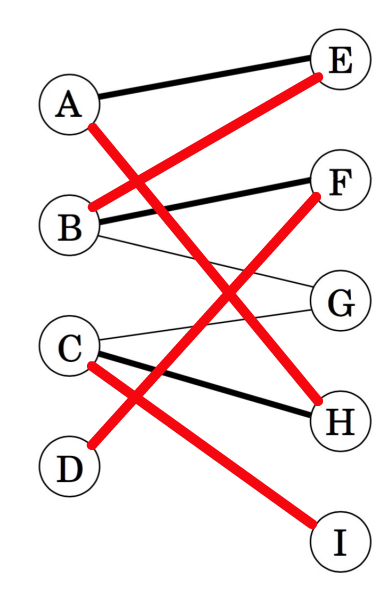
\includegraphics[width=0.4\textwidth]{alternatepath}

\item
Add a source and sink node to the graph.\\
Connect the unmatched nodes on the Left side to the source.\\
Connect the unmatched nodes on the right side to the sink.\\
For each edge in M, add a directed edge from R to L.\\
For each edge in E-M, add a directed edge from L to R.\\
Find a path from s-t.\\
Correctness: Any path from s-t on this graph is necessarily an alternating path, even just an unmatched edge that connects s - t for a length of 3. An alternating path requires that an unmatched edge be chosen fist, and then alternate between a matched and unmatched edge. The algorithm ensures this because we made all of the matched edges in M point from Right to left, or simply put, backwards. Thus, to get a correct path, we need to alternate from unmatched to matched.\\ 
\item
Connect all of the Left nodes to the source\\
Connect all of the right nodes to the sink\\
Make all capacities 1\\
Run Ford-Fulkerson on this graph.
The edges from L to R that are set to 0, are the maximal matching.\\
Correctness: Since all of the capacities are 1, the maximum flow is equivalent to the number of edges between L and R. The Ford-Fulkerson algorithm will find the largest flow, and therefore, the maximal matching. This algorithm runs in $O(|V| \cdot |E|)$ because in the worst case, it will explore all nodes and edges in the graph.
\end{enumerate}

\item {\bf (Extra Credit)}
We want to analyze the economic dependence between $n$ provinces in a
country. A province $i$ has an annual budget surplus $s_i$, which may be
positive or negative. Moreover, for any $1\leq i,j\leq n$, let
$e_{ij}$ be the total annual value of exports from province $i$ to
province $j$ (has to be nonnegative). Is there a strict subset $S$ (of
size less than $n$)  of provinces such that the total budget surplus
in $S$ is at least as much as the total export out of $S$? Give a
polynomial time algorithm for this problem. Establish its correctness and
time complexity.
\textbf{Solution:}\\
Each province is a node in a graph.\\
Add a source and a sink.\\
Connect every province $i$ to the source, each having a capacity of $s_i$.\\
Connect every province $j$ to the sink, each having a capacity of $s_j$.\\
The edges that connect province i to j, has a capacity $e_{ij}$.\\
Run Ford-Fulkerson on the resulting graph.
Correctness: Running Ford-Fulkerson will maximize the total budget surplus coming from the source, i.e. maximizing flow. The total budget surplus in subset S will be  equivalent to the min cut. Therefore the total budget surplus will be at least as large as the total export. 
\end{enumerate}


\end{document}